\documentclass[9pt,twocolumn,letterpaper]{article}

\usepackage{cvpr}
\usepackage{times}
\usepackage{epsfig}
\usepackage{graphicx}
\usepackage{amsmath}
\usepackage{amssymb}
\usepackage{array,multirow,makecell}
\usepackage{pstricks}

% Include other packages here, before hyperref.

% If you comment hyperref and then uncomment it, you should delete
% egpaper.aux before re-running latex.  (Or just hit 'q' on the first latex
% run, let it finish, and you should be clear).
\usepackage[breaklinks=true,bookmarks=false]{hyperref}
\usepackage[margin=2.2cm,top = 2cm, bottom = 2cm, includefoot]{geometry}

\cvprfinalcopy % *** Uncomment this line for the final submission

\def\cvprPaperID{****} % *** Enter the CVPR Paper ID here
\def\httilde{\mbox{\tt\raisebox{-.5ex}{\symbol{126}}}}

% Pages are numbered in submission mode, and unnumbered in camera-ready
%\ifcvprfinal\pagestyle{empty}\fi
\setcounter{page}{1}
\begin{document}

%%%%%%%%% TITLE
\title{Report TP1 -  Speech Commands}

\author{Philippe Ganshof\\
ENS Paris-Saclay\\
94230 Cachan\\
{\tt\small philippe.ganshof@hotmail.com}
% For a paper whose authors are all at the same institution,
% omit the following lines up until the closing ``}''.
% Additional authors and addresses can be added with ``\and'',
% just like the second author.
% To save space, use either the email address or home page, not both
}

\maketitle
%\thispagestyle{empty}

%%%%%%%%% ABSTRACT
%\begin{abstract}
   %%The ABSTRACT is to be in fully-justified italicized text, at the top
   %of the left-hand column, below the author and affiliation
   %information. Use the word ``Abstract'' as the title, in 12-point
   %Times, boldface type, centered relative to the column, initially
   %capitalized. The abstract is to be in 10-point, single-spaced type.
   %Leave two blank lines after the Abstract, then begin the main text.
   %Look at previous CVPR abstracts to get a feel for style and length.
%\end{abstract}

%%%%%%%%% BODY TEXT




\section{Introduction}
We studied in this practical work how to classify voice commands recorded by devices such as Amazon Alexa. The dataset consists of 1 second voice commands stored as waveforms. In a first time, we extracted the Mel-log filterbanks and MFCC speech features and evaluated how the different settings influence the validation performance. We then used our language model to predict sequences of voice commands and compared three different methods, the Greedy, Beam and Viterbi search algorithms.




\section{Classification of segmented voice commands}
The goal of this part was to analyse the influence of different settings on the performance of the classification task. As a quantitative measure, we computed the accuracy on a validation set consisting of 1000 examples. In the first three questions, we focused on finding optimal parameters for the speech features. Using these parameters, we then studied different transformations on the dataset such as normalisation. Finally, we focused on the classifier and compared three different models. This lead us to find an optimal configuration with which we analysed the classes that are the most difficult to find. It is also important to note that the accuracy vary between some questions (in particular questions 1-2,3,4-5-6) because the initial value of the model changes over time, even tough the random seed stays the same.

 

\subsection{Question 1.1: Frequency range}
To quantitatively measure the influence of the frequency range on the validation performance, we first fixed the lower limit and let the higher limit vary. We then followed the same reasoning but this time keeping the higher limit fixed. Our results are illustrated in figure 1 and we can see with the right graph that frequencies between 0 and 3000 play an important role in the performance of the model. This concords with the human speech characteristics as the voice frequency lies between the same range approximatively. On the left graph, the accuracy keeps increasing even after 3000Hz which was not expected. However, the fact that we get an accuracy near zero if we do do include frequencies between 0 and 3000Hz does tell us that the signals useful for our classification task lie in this particular range. We also note that setting the lower frequency limit to zero does not lead to the best results. I believe that when we start at 100 or 500, it removes part of the low frequency noise and thus improves the validation performance. The best accuracy we obtained on the validation set was with range 500Hz to 5500Hz.

\begin{table}
\begin{center}
\begin{tabular}{|c|c|c|c|}
\hline
 First $\backslash$ Second & False & True\\
 \hline
 False & 41.5\% & 39\%\\
 \hline
 True & 46.5\% & 41.4\% \\
 \hline
\end{tabular}
\end{center}
\caption{{\bf Influence of first and second derivatives.} We modify the presence or absence of first and second derivatives of the cepstral coefficients in the speech features and measure the accuracy on the validation set.}
\end{table}

\subsection{Question 1.2: Mel-Log Filterbanks and MFCC}
By changing the number of filters for the mel-log filterbanks features, we obtained very odd results difficult to interpret. We let the number of filters vary between 10 and 40 as suggested in the literature to accurately capture how much energy occurs at each spot. The accuracy was close to zero (or zero) most of the times expect for some peak values at 13, 29 and 39, see figure 2. The role of these filters is usually to reject the unwanted frequencies with no useful signal energy but in this case, the gathered information totally mislead the classifier.\par
We then fixed the number of filters and let the number of cepstral coefficients for the MFCC speech features vary between 2 and 16, illustrated in figure 2. We can see that the peak performances lie between 4 and 8 and then the accuracy tends to decrease which gives us a good indication on how to choose this paramater. This supports the explanation seen in the lecture that the firsts coefficients in the cepstral domain capture most of the vocal tract resonance. We also note that the number of filters has a relatively low influence on the validation performance when it lies between 20 and 60. The best accuracy we obtained on the validation set is with 40 filters and 6 cepstral coeffcients.

\begin{figure*}
\begin{center}
\includegraphics[width=1\linewidth]{graph.png}
\end{center}
   \caption{{\bfseries Validation performance according to frequency range.} On the left graph, we fixed the the lower frequency limit at four different values, 0, 100, 500 and 1000 respectively and let the higher limit vary. The right graph is similar but this time the lower limit varies while the higher limit remains fixed. Again, we repeat the process with four different higher frequency limit representing the different colours, 7500, 7000, 6000 and 5000 respectively. }
\label{fig:short}
\end{figure*}
\begin{figure*}
\begin{center}
\includegraphics[width=1\linewidth]{graph2.png}
\end{center}
   \caption{{\bfseries Validation performance according the number of filters and cepstral coefficients.} On the left graph, we let the number of filters for the Mel-log filterbank speech features vary between 10 and 40. On the right graph, we fix the number of filters at three different values 20, 40 and 60 and let the number of cepstral coefficients for the MFCC speech features vary with jumps of 2 between 2 and 16.}
\label{fig:short}
\end{figure*}

\begin{table}
\begin{center}
\scalebox{0.85} & 63.3\% & 54.4\% & 61.1\%\\
 \cline{3-5}
Across-Channel &     & 20.1\%   & 17.5\%  & 19.4\%\\
\hline
\end{tabular}}
\end{center}
\caption{{\bf Influence of Normalisation.} We compare the accuracy on the validation set with three different normalisation methods, per- and across channel.}
\end{table}

\subsection{Question 1.3: Delta and delta delta for MFCC}
In order to measure the influence of the presence or absence of the first and second derivative of the cepstral coefficients in the speech features, we simply try the four different possibilities and analyse the impact on the validation performance.  As we can see in table 1, one configuration stands out, when we consider the first but not the second derivatives. We also note that the presence of the first derivatives improves the accuracy independently of the second derivatives.

\subsection{Question 1.4: Pre-processing methods}
After having found our optimal parameters for speech features, we look at some pre-processing techniques that could improve the accuracy on the validation set such as normalisation or modifying the training size. We also study the robustness of our model by adding noise to the waveforms of the training set.\par We tested three different normalisation methods per- and across channel:\\
[2mm]
(1) Method 1: Dividing each speech features vector by its maximum element.\\
[2mm]
(2) Method 2: Dividing each speech features vector by its L2 norm.\\
[2mm]
(3)  Method 3: Scale each speech features vector to have mean 0 and variance 1.\\
[2mm]
We can see in table 2 that per-channel normalisation has a strong beneficial effect for all three methods. Such results were expect as normalisation is a usual task when processing the data in machin learning. Normalisating the data brings many advantages such as taking less space and should be used in our case.  Method 1 and 3 seems to produce better results but the related performance improvement has high volatility and so Method 2 should not to be left out for future analysis. On the other hand, across channel normalisation leads to poor results as expected. Indeed, normalising across channel makes speech features vectors inter-dependent and we thus lose information.\par
By adding 100 examples of each label in the training size, we were able to increase the accuracy by 1.9\%. As the table shows, further increasing the training size does not necessarily leads to an improvement in the performance as it is more likely to overfit the training data.\par
Finally, we inserted a gaussian noise on the dataset to check the robustness of our model. For each training wave, we added a standard gaussian noise of the same size and the accuracy fell from 43.6\% to 21.7\% as expected. Further work is needed to improve the stability of the model.



\begin{table}
\begin{center}
\begin{tabular}{|c|c|c|c|c|}
\hline
 Training size & 6000& 9000 &  12000 &  15000 \\
 \hline
Accuracy & 41.6\% & 43.6\% & 45.5\% & 42.1\% \\
 \hline
\end{tabular}
\end{center}
\caption{{\bf Influence of Training size.} We compare the accuracy on the validation set with four different training sizes.}
\end{table}

\subsection{Question 1.5: Model$'$s choice and hyper-parameters }
The last step to find an optimal configuration consists of choosing the right model for the classification task. We tested the validation performance of three models, the Logistic Regression, Multi-layer Perceptron and the SVM, using different hyperparameters as shown in tables 4,5 and 6. Our analysis is biased towards the Multi-layer Perceptron as the optimal parameters deduced from the previous parts is based on this model. We obtained far better results with the Multi-layer Perceptron attaining an accuracy of 60.9\% on the validation set. A better model could be built using convolutional neural networks since they take advantage of the high correlation between the frequencies in the neighbours windows.

\subsection{Question 1.6: Best model}
The results obtained in the previous questions lead us to choose the following configuration:
\begin{flushleft}
Speech features for MFCC settings:\\
[2mm]
- Frequency range: From 500Hz to 5500Hz\\
[2mm]
- Number of filters: 40\\
[2mm]
- Number of cepstral coefficients: 6\\
[2mm]
- Delta = True and DeltaDelta = False\\
[2mm]
Pre-processing methods:\\
[2mm]
- Normalisation method 1\\
[2mm]
- Extend the training size to 400 examples per labels\\
[2mm]
Multi-Layer Perceptron settings:\\
[2mm]
- Learning rate set at 0.01\\
[2mm]
- 1 Hidden layers with 130 units\\
[2mm]
- regularisation parameter set as 1e-2
\end{flushleft}
Our modifications led to a drastic improvement over the original configuration. The normalisation method and the choice of the model mainly contributed to such an increase on the validation accuracy.\par
In order to analyse the classes that are the most difficult to find for our model, we built a confusion matrix on the train set and an extended validation set (not the validation set used before as it is only containing 5 labels but a validation set containing 40 examples of each class) shown in figures 3 and 4. The value in each box for a point (word1,word2) correspond to the percentage of times the word2 has been predicted when word1 has been given as input. We see that our model often confuses the word $\textit{three}$ with $\textit{tree}$ for example which makes sense from a phonetic point of view. However, the model also often confuses the words \textit{no} and \textit{down} which shows inconsistency in some cases. Overfitting is illustrated with the diagonal terms since they are significantly higher in the confusion matrix on the training set. A regularisation methods such as dropout could be used to get better generalisation.


\begin{table}
\begin{center}
\scalebox{0.75}{%
\begin{tabular}{|c|c|c|c|c|c|c|}
\hline
 Regularisation constant& 0.1 & 1 &  10 &  100 & 1e3 & 1e4 \\
 \hline
Accuracy & 24.9\% & 29\% & 28.1\% & 28.8\%  &28.9\% & 29.1\\
 \hline
\end{tabular}}
\end{center}
\caption{{\bf Logistic Regression.} We tested the logisitic regression model on the validation set with different regularisation constants.}
\end{table}

\begin{table}
\begin{center}
\scalebox{0.72}{%
\begin{tabular}{|c|c|c|c|c|c|c|}
\hline
 Regularisation constant& 1e-6 & 1e-5 &  1e-4 & 1e-3 & 1e-2 & 1e-1 \\
 \hline
Accuracy & 11.7\% & 13.4\% & 7.1\% & 27.7\%  &14.5\% & 1.6\%\\
 \hline
\end{tabular}}
\end{center}
\caption{{\bf SVM.} We tested the support vector machine model on the validation set with different regularisation constants.}
\end{table}

\begin{table*}
\begin{center}
\scalebox{0.9}{%
\begin{tabular}{|c|c|c|c|c|c|c|c|c|c|c|c|c|}
\hline
 Alpha $\backslash$ Num HiddLayers &50 & 60 & 70  & 80 & 90 & 100 & 110 & 120 & 130 & 140 & 150\\
 \hline
 1e-5 & 49.3\% & 46.3\%     & 48.6\% &   47.1\%  & 46.9\%    & 48.1\% & 46\%  & 48.5\%  & 56.1\%  & 54.1\%  & 51.5\%\\
 \hline
 1e-4 & 49.4\% & 42.7\%   & 43.6\%  & 48.4\%     &  52.8\%   & 51.8\%    & 48.3\%   & 53.3\%  & 55\%   & 50\%& 53\% \\
 \hline
 1e-3 &  52.9\%  & 54.4     & 51.6\%    & 53.6\%    &  49.6\%     & {\bf 57.3\%}    & 48.9\%   &  47.2\%  & 56.7\%    & 53.7\%  & 54.6\%\\
 \hline
 1e-2 &   {\bf 60.9\%}  &  49.1\%  & 48.7\%   &   56\%\    & 54.9\% &  52.5\%  &   {\bf 58.5\%}   & 55.8\%  & {\bf 60\%}   & 57.1\%  & {\bf 58.1\%}\\
 \hline
 1e-1 &    43.3\%   &  52.7\% & 43.6\%    & 43.8\% &  53.5\%    &  50.2\%   &     47.6\%     &  51.9\%  & 52.8\%   & 52.1\% & 47.2\%\\
 \hline
 1 &      25.6\%       &   34.5\%   & 34.7\%     &  41.5    & 39.2\%   &  35.8\%   &  29.3\%   &   38.7\%   & 32.3\%  & 30.9\% & 34.4\%\\
 \hline
\end{tabular}}
\end{center}
\caption{{\bf Multi-layer Perceptron.} We tested the Multi-layer Perceptron model on the validation set with pairs consisting of the regularisation parameter and the number of hidden layers. We pointed out in bold the pairs leading to the best generalisations. }
\end{table*}


\begin{figure*}
\begin{center}
\scalebox{1}{%
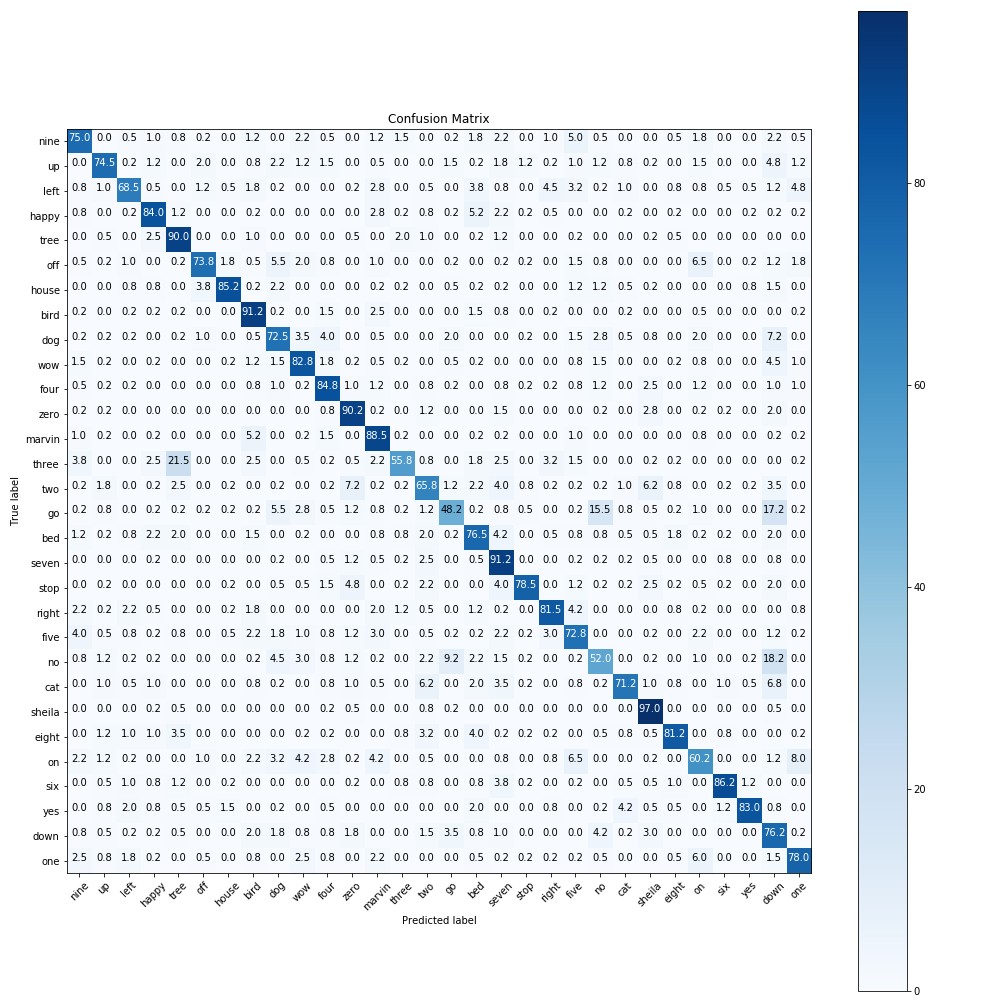
\includegraphics[width=1\linewidth]{confusion_matrix1.png}}
\end{center}
   \caption{{\bfseries Confusion matrix on the train set.} }
\label{fig:short}
\end{figure*}
\newpage


\begin{figure*}
\begin{center}
\scalebox{1}{%
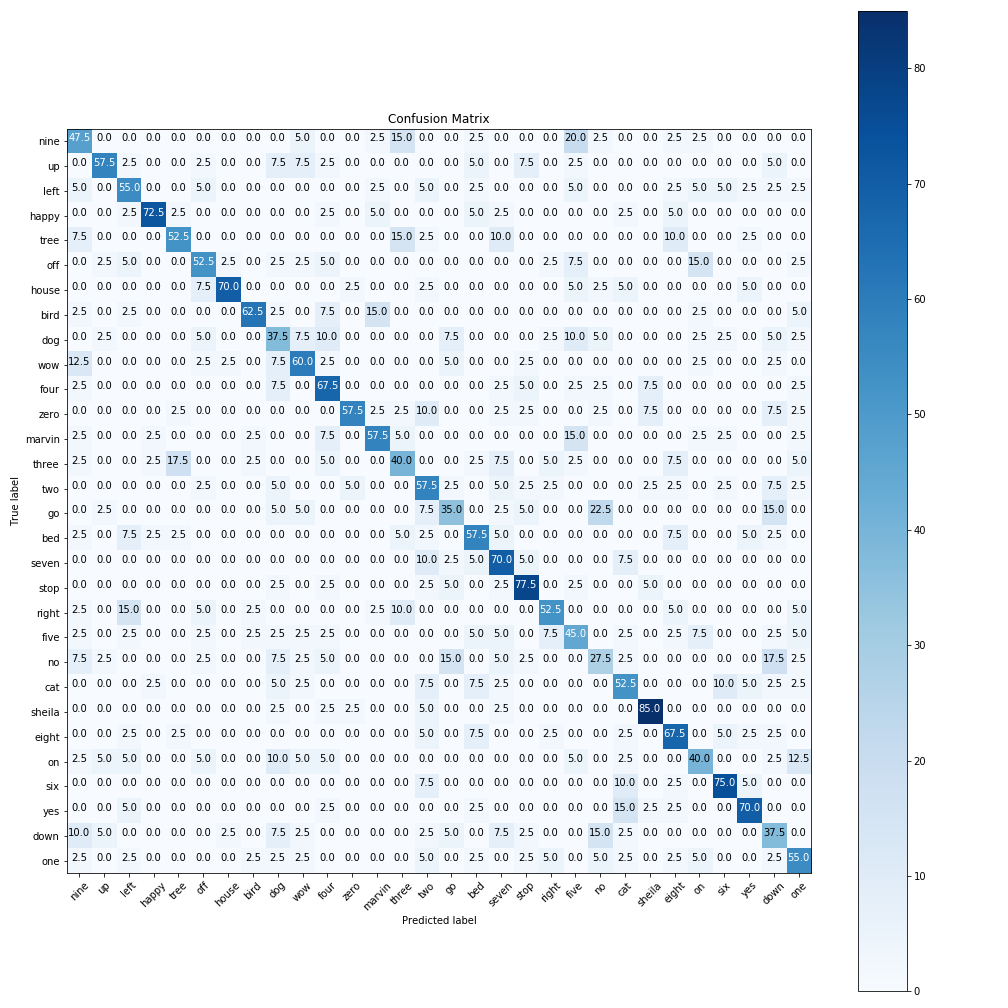
\includegraphics[width=1\linewidth]{confusion_matrix2.png}}
\end{center}
   \caption{{\bfseries Confusion matrix on an extended validation set.} }
\label{fig:short}
\end{figure*}
\newpage


\section{Prediction of Sequences}
In this part, we implemented and compared three differrent methods for predicting sequences of voice commands.
\subsection{Question 2.1}
In the cells where we build our training dataset, each class is equally represented, so we put a uniform prior on the vocabulary. We thus assumed that there are no words rarer than others in the language which is in practice obviously not true. More precisely, this was done at line:\\
$$\text{elif train\_labels.count(label)} < \text{nb\_ex\_per\_class}$$

\subsection{Question 2.2}
Since S,D,I,N are non-negative integers, the word error rate cannot be strictly negative. However, it can exceed 100 as shown in the following example: When "I eat a sweet apple" is decoded as "I ate a little green turtle with you", then $N = 5$, $S = 3$, $I = 3$, $D = 0$ which gives us $WER = 100\frac{3 + 3 + 0}{5} = 125$.

\subsection{Question 2.3}
We consider the following example:
\begin{center}
Reference sentence: go marvin one right stop\\
[2mm]
Predicted sentence with greedy search: go five one up stop
\end{center}
The number of substitutions equals $2$, \textit{marvin} and \textit{right} are wrongly decoded as \textit{five} and \textit{up} respectively. Since both sentences have same length, $I = D = 0$ and $N = 5$ as the reference sentence is of length $5$. This gives us $WER = 0.4$.

\subsection{Question 2.4}
Bigram model correspond to the following assumption on the language model:\\
[2mm]
$$ P(W) = \prod_{k=1}^{L} P(W_{k} | W_{k-1}) \eqno (1)$$


 
\subsection{Question 2.5}
We stored the conditional probabilities of each pair of words $(w1,w2)$ in a $31\text{x}30$ matrix (30 corresponding to the number of words in the vocabulary and 31 same but with the "first word" which has been added at the beginning of each sentence). To compute\\
$$ P(W1 | W2) = \frac{c(W1,W2)}{c(W2)},$$
$$W1,W2 = \text{"Words in the vocabulary"}$$
we counted the number of sentences in the training list containing the sequence W2W1 (c(W1,W2)) for each pair of words and then normalised by the sum of the rows (divided by c(W2), the number of sentence containing the word W1)). Since $P(W1 | W2)$ often equals zero, it leads to data sparsity and to avoid that, we added a constant $1$ to each term in the matrix. This method is called Laplace smoothing. We also added the word "$<d>$" at the beginning of each sentence to be able to condition the "real" first word on this new added word.

\begin{table}
\begin{center}
\scalebox{0.85}{%
\begin{tabular}{|c|c|c|c|c|}
\hline
  & Greedy search & Beam search & Viterbi search\\
 \hline
Subset of train set & 0.52& 0.37 & 0.42  \\
 \hline
 Test set & 0.48 & 0.33 & 0.32 \\
 \hline
\end{tabular}}
\end{center}
\caption{{\bf Word Error Rate.} We compare the Greedy, Viterbi and Beam search on the test set and a subset of the train set containing 300 elements}
\end{table}

\subsection{Question 2.6}
As we increase $N$ (the number of previous words we take in account when computing conditional probabilities), we get a better approximation of the language model because we get "closer" to the Baye's rule. However, the number of elements in the tensor is given by $M^{N}$ where $M = \text{Number of words in the vocabulary}$ and thus increases exponentially in $N$.  This makes the matrix very sparse as a huge amount of sentences is needed in the training set to get non-zero values. The consequences of sparsity are explained in question 2.10.
\subsection{Question 2.7}
We deduce from our implementation of the beam search algorithm that the time complexity equals $\mathcal{O}(LBW + L(BW\text{log}(BW))) = \mathcal{O}(LBW ( 1 + \text{log}(BW))$. We assumed that the time complexity for sorting an array of size $n$ was $\mathcal{O}(n\text{log}(n))$ and we used the following notations:
\begin{center}
W = "Number of words in the vocabulary"\\
[2mm]
B = "Width of Beam search"\\
[2mm]
L = "Sequence Length"
\end{center}
The working memory has complexity $\mathcal{O}(BWL).$

\subsection{Question 2.8}
If $f_{k}(j)$ denotes the probability to be in state j at step k, then we have the following formula:
\begin{center}
$$ f_{k}(j) = \underset{i \in \lbrace 1,...,30 \rbrace}{\text{max}}  p(w_{k} = j | w_{k-1} = i) f_{k-1}(i) $$
$$ f_{2}(i) = A_{i,31} \:\:\: \text{(31 being the index of the "first word")}  $$
\end{center}
where $p(w_{k} = j, w_{k} = i) = A_{i,j}$ and $A_{i,j}$ denotes the transition matrix. Note that here, the index set associated with the labels starts at 1. The complexity of the algorithm equals $\mathcal{O}(LW^{2})$.

\subsection{Question 2.9}
As expected Beam and Viterbi search perform much better than the greedy search as they use in a smart way the previous words to predict the next one. Viterbi algorithm is in theory better than the Beam search. The Viterbi gives the sequence of words maximising (1) in contrast with the outputs of Beam search which do not necessarily maximise (1) because some solutions are neglected. This is confirmed with Table 7 where we see that Viterbi algorithm leads to a better WER on the test set. However, this is not the case on the subset of the train set.

\begin{table}
\begin{center}
\scalebox{0.82}{%
\begin{tabular}{|c|c|c|c|c|}
\hline
  & & Without Smoothing & Laplace Smoothing\\
\hline
 \multirow{2}{1cm}{Beam} & sub strain set & 0.38 & 0.37\\
  & test set & 0.38 & 0.33\\
\hline
\multirow{2}{1cm}{Viterbi} & sub train set & 0.44 & 0.42\\
& test set & 0.36 & 0.32\\
\hline

 \end{tabular}}
\end{center}
\caption{{\bf Word Error Rate.} We compare the Viterbi and Beam search on the test set and a subset of the train set containing 300 elements with and without smoothing.}
\end{table}


\subsection{Question 2.10}
By predicting several sequences with the Beam and Viterbi search algorithms, we noticed that these models fail to prevent the confusion (and so make use of the sentence structure) when a pair of words has a high confusion rate in the confusion matrix. For example, if the reference sentence is $\textit{up on right}$, the algorithms will often predict $\textit{five}$ instead of $\textit{on}$ which gives us $\textit{up five right}$.\\
If we do not use Laplace smoothing, then the bigram matrix becomes very sparse and some words will never be predicted if they do not appear often in the training sentences since the conditional probabilities associated to this word will equal zero.

\subsection{Question 2.11}
As we explained in Question 2.5 and 2.10, Laplace smoothing is a good technique to face the problem of rare seen words. We can see on table 8 that the WER on the validation set decreases when we use Laplace smoothing which supports our argumentation.

\subsection{Question 2.12}
To jointly train an acoustic and a language model, we can use the end-to-end speech recognition approach. Indeed, the problem can be seen as a sequence-to-sequence model where the input is an acoustic characteristic and the output a text sequence. Thus one can use recurrent neural networks such as LSTM or better, an attention-based encoder-decoder framework. A reference that explains how to do so can be found below.



\begin{thebibliography}{4}

\bibitem{J18}
Zhengkun Tian, Jiangyan Yi, Jianhua Tao, Ye Bai, and Zhengqi Wen,
\newblock{Self-attention transducers for
end-to-end speech recognition},
\newblock{Interspeech 2019, Sep 2019.}



\end{thebibliography}



















\end{document}
